%%%%%%%%%%%%%%%%%%%%%%%%%%%%%%%%%%%%%%%%%
% Make sure to set your name, legi number and url to the right git branch.
\newcommand{\hmwkAuthorName}{Michiels Joran} % Your name
\newcommand{\hmwkAuthorLegi}{16-948-549} % Your name
\newcommand{\hmwkGitBranch}{16-948-549/1\_locally\_linear\_embedding} % Your name
%
%%%%%%%%%%%%%%%%%%%%%%%%%%%%%%%%%%%%%%%%%

%----------------------------------------------------------------------------------------
%	PACKAGES AND OTHER DOCUMENT CONFIGURATIONS
%	Skip this
%----------------------------------------------------------------------------------------

\documentclass{article}

\usepackage{fancyhdr} % Required for custom headers
\usepackage{lastpage} % Required to determine the last page for the footer
\usepackage{extramarks} % Required for headers and footers
\usepackage{graphicx} % Required to insert images
\usepackage{lipsum} % Used for inserting dummy 'Lorem ipsum' text into the template

% Margins
\topmargin=-0.45in
\evensidemargin=0in
\oddsidemargin=0in
\textwidth=6.5in
\textheight=9.0in
\headsep=0.25in 

\linespread{1.1} % Line spacing

% Set up the header and footer
\pagestyle{fancy}
\lhead{\hmwkAuthorName} % Top left header
\chead{\hmwkClass\ \hmwkTitle} % Top center header
\rhead{\firstxmark} % Top right header
\lfoot{\lastxmark} % Bottom left footer
\cfoot{} % Bottom center footer
\rfoot{Page\ \thepage\ of\ \pageref{LastPage}} % Bottom right footer
\renewcommand\headrulewidth{0.4pt} % Size of the header rule
\renewcommand\footrulewidth{0.4pt} % Size of the footer rule

\setlength\parindent{0pt} % Removes all indentation from paragraphs

%----------------------------------------------------------------------------------------
%	DOCUMENT STRUCTURE COMMANDS
%	Skip this
%----------------------------------------------------------------------------------------

% Header and footer for when a page split occurs within a problem environment
\newcommand{\enterProblemHeader}[1]{
\nobreak\extramarks{#1}{#1 continued on next page\ldots}\nobreak
\nobreak\extramarks{#1 (continued)}{#1 continued on next page\ldots}\nobreak
}

% Header and footer for when a page split occurs between problem environments
\newcommand{\exitProblemHeader}[1]{
\nobreak\extramarks{#1 (continued)}{#1 continued on next page\ldots}\nobreak
\nobreak\extramarks{#1}{}\nobreak
}

\setcounter{secnumdepth}{0} % Removes default section numbers
\newcounter{homeworkProblemCounter} % Creates a counter to keep track of the number of problems

\newcommand{\homeworkProblemName}{}
\newenvironment{homeworkProblem}[1][Problem \arabic{homeworkProblemCounter}]{ % Makes a new environment called homeworkProblem which takes 1 argument (custom name) but the default is "Problem #"
\stepcounter{homeworkProblemCounter} % Increase counter for number of problems
\renewcommand{\homeworkProblemName}{#1} % Assign \homeworkProblemName the name of the problem
\section{\homeworkProblemName} % Make a section in the document with the custom problem count
\enterProblemHeader{\homeworkProblemName} % Header and footer within the environment
}{
\exitProblemHeader{\homeworkProblemName} % Header and footer after the environment
}

\newcommand{\problemAnswer}[1]{ % Defines the problem answer command with the content as the only argument
\noindent\framebox[\columnwidth][c]{\begin{minipage}{0.98\columnwidth}#1\end{minipage}} % Makes the box around the problem answer and puts the content inside
}

\newcommand{\homeworkSectionName}{}
\newenvironment{homeworkSection}[1]{ % New environment for sections within homework problems, takes 1 argument - the name of the section
\renewcommand{\homeworkSectionName}{#1} % Assign \homeworkSectionName to the name of the section from the environment argument
\subsection{\homeworkSectionName} % Make a subsection with the custom name of the subsection
\enterProblemHeader{\homeworkProblemName\ [\homeworkSectionName]} % Header and footer within the environment
}{
\enterProblemHeader{\homeworkProblemName} % Header and footer after the environment
}
   
%----------------------------------------------------------------------------------------
%	NAME AND CLASS SECTION
%	Skip this
%----------------------------------------------------------------------------------------

\newcommand{\hmwkTitle}{Locally Linear Embedding} % Assignment title
\newcommand{\hmwkDueDate}{Monday,\ March\ 6th,\ 2017} % Due date
\newcommand{\hmwkClass}{SLT coding exercise\ \#1} % Course/class
\newcommand{\hmwkClassTime}{Mo 16:15} % Class/lecture time
\newcommand{\hmwkClassInstructor}{} % Teacher/lecturer

%----------------------------------------------------------------------------------------
%	TITLE PAGE
%	Skip this
%----------------------------------------------------------------------------------------

\title{
\vspace{2in}
\textmd{\small{\hmwkClass}}\\
\textmd{\textbf{\hmwkTitle}}\\
\small{https://gitlab.vis.ethz.ch/vwegmayr/slt-coding-exercises}\\
\normalsize\vspace{0.1in}\small{Due\ on\ \hmwkDueDate}
%\vspace{0.1in}\large{\textit{\hmwkClassInstructor\ \hmwkClassTime}}
\vspace{3in}
}

\author{
\hmwkAuthorName\\
\hmwkAuthorLegi
}

\date{ } % Insert date here if you want it to appear below your name

\begin{document}

\maketitle

%----------------------------------------------------------------------------------------
%	TABLE OF CONTENTS
%	Skip this
%----------------------------------------------------------------------------------------

%\setcounter{tocdepth}{1} % Uncomment this line if you don't want subsections listed in the ToC

\newpage
\tableofcontents
\newpage

%----------------------------------------------------------------------------------------
%	SECTIONS
%	Now you are in the right hood
%----------------------------------------------------------------------------------------

\begin{homeworkProblem}[The Model]
The model section is intended to allow you to recapitulate the essential ingredients used in \hmwkTitle. Write down the \textit{necessary} equations to specify \hmwkTitle\ and and shortly explain the variables that are involved. This section should only introduce the equations, their solution should be outlined in the implementation section.\newline
Hard limit: One page
\vspace{10pt}

\problemAnswer{ % Answer
In Locally Linear Embedding the goal is to represent a data set of \textit{N} points $\textbf{x}_i \in \Re^D$ in a low dimensional space $\Re^d$ ($\textbf{y}_i \in \Re^d$) with $d \ll D$. It is assumed that the data points (dimension \textit{D}) lie (approximately) on a manifold of dim \textit{d}. 
\bigskip \par

First the nearest neighbours for every $\textbf{x}_i$ have to be found (denoted by $\textbf{x}_j$). Out of these points, $\textbf{x}_i$ can be approximately reconstructed. The best weights $\textit{w}_{ij}$ can be found by minimizing the following error:

\begin{equation} \label{eq:1}
E(W)=\sum_{i} \| \textbf{x}_i -\sum_{j}\textit{w}_{ij} \textbf{x}_j  \|
\end{equation}

under the constraints $\sum_{j}\textit{w}_{ij} = 1$. $\textit{w}_{ij}$ is zero when $\textbf{x}_j$ is not a nearest neighbour of $\textbf{x}_i$.
\bigskip \par

Note that these weights are invariant to rotations, rescalings and translations of the data point and it's neighbours. These weights represent the local geometry of the data space. When the data (approximately) lies on a manifold of dimension \textit{d}, it is expected that the local geometry of small patches will be equal to the local geometry of the original data space. Therefore the weights $\textit{w}_{ij}$ can be reused. 
\bigskip \par

The points $\textbf{y}_i \in \Re^d$ can then be found by minimizing the cost function:

\begin{equation} \label{eq:2}
E(Y)=\sum_{i} \| \textbf{y}_i -\sum_{j}\textit{w}_{ij} \textbf{y}_j  \|.
\end{equation}
}
\end{homeworkProblem}
\clearpage

%----------------------------------------------------------------------------------------
\begin{homeworkProblem}[The Questions]
This is the core section of your report, which contains the tasks for this exercise and your respective solutions. Make sure you present your results in an illustrative way by making use of graphics, plots, tables, etc. so that a reader can understand the results with a single glance. Check that your graphics have enough resolution or are vector graphics. Consider the use of GIFs when appropriate.\newline
Hard limit: Two pages

\begin{homeworkSection}{(a) Get the data}
For this exercise we will work with the MNIST data set. In order to learn more about it and download it, go to http://yann.lecun.com/exdb/mnist/.
\end{homeworkSection}

\begin{homeworkSection}{(b) Locally linear embedding}
Implement the LLE algorithm and apply it to the MNIST data set. Provide descriptive visualizations for 2D \& 3D embedding spaces. Is it possible to see clusters?
\end{homeworkSection}

\begin{homeworkSection}{(c) Cluster structure}
Investigate the cluster structure of the data. Can you observe block structures in the $M$ matrix (use matrix plots)? Also plot the singular values of $M$. Do you notice something?
Can you think of ways to determine the optimal embedding dimension?
\end{homeworkSection}

\begin{homeworkSection}{(d) Nearest Neighbors}
Investigate the influence of the choice of how many nearest neighbors you take into account. Additionally, try different metrics to find the nearest neighbors (we are dealing with images!).
\end{homeworkSection}

\begin{homeworkSection}{(e) Linear manifold interpolation}
Assume you pick some point in the embedding space. How can you map it back to the original (high dimensional) space? Investigate how well this works for points within and outside the manifold (does it depend on the dimensionality of the embedding space?) Try things like linearly interpolating between two embedding vectors and plot the sequence of images along that line. What happens if you do that in the original space?
\end{homeworkSection}

\vspace{10pt}
\problemAnswer{ % Answer
\bigskip

\begin{homeworkSection}{(b) Locally linear embedding}
\begin{center}
	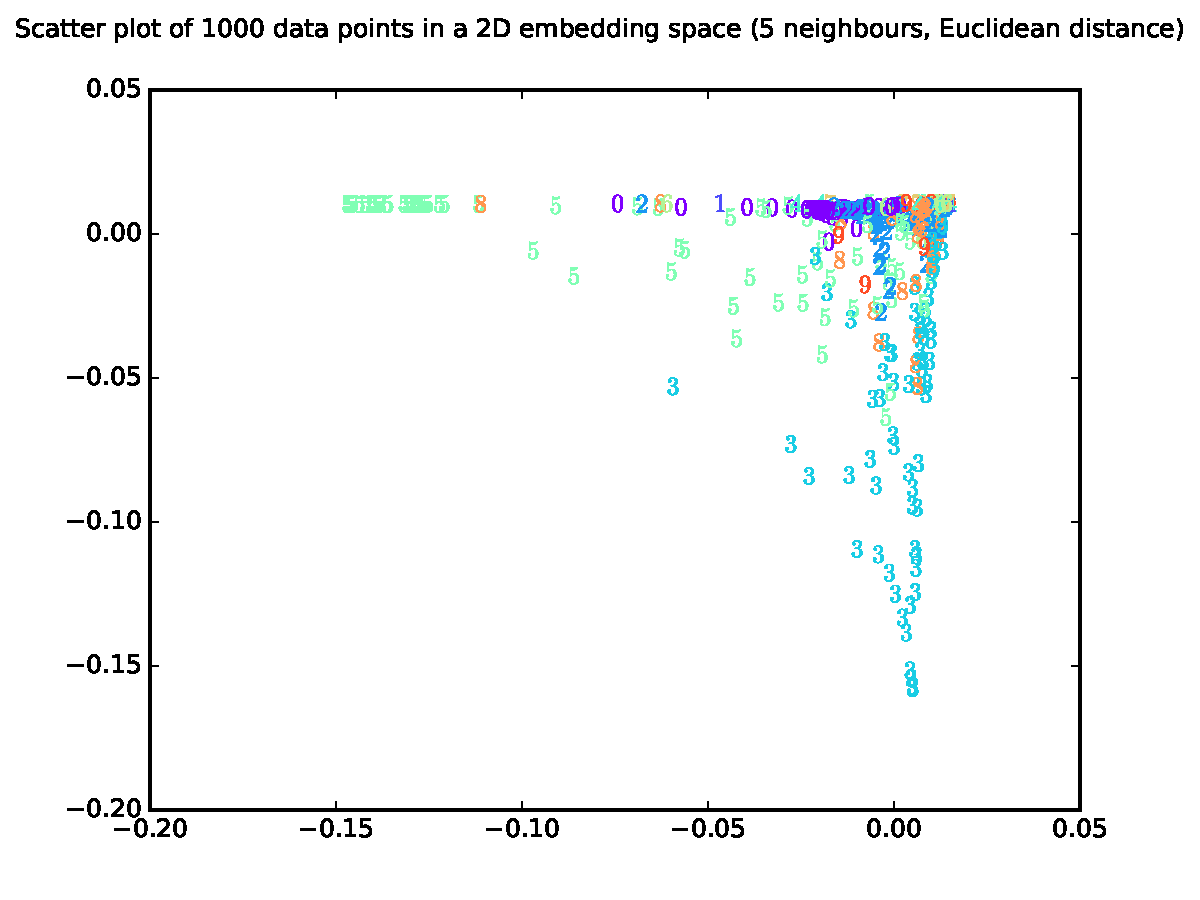
\includegraphics[scale=0.6]{1_figures/2Dembed_5neigh_Euclidean}
\end{center}
\begin{center}
	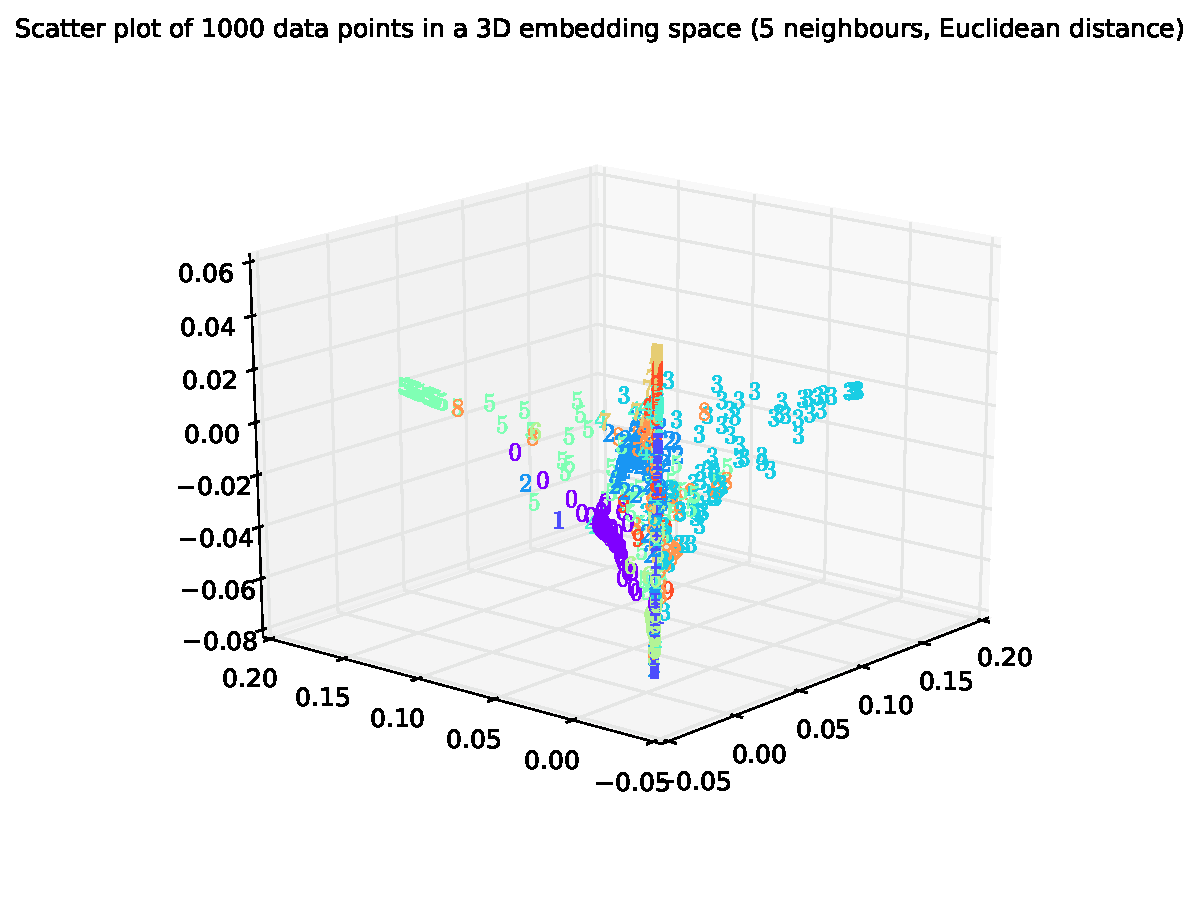
\includegraphics[scale=0.6]{1_figures/3Dembed}
\end{center}
The above results are for 5 neighbours using the Euclidean distance.
It is possible to see a bit of clustering, although it is easier for some numbers (labels) than for others (e.g. the number 5 vs 1). In the 3D embedding space some clusters are better to see (e.g. the number 0).
\end{homeworkSection}
}

\problemAnswer{ % Answer
\bigskip

\begin{homeworkSection}{(c) Cluster structure}
The structure of the matrix \textit{M} is symmetric with a dominant diagonal. This follows from its construction:
\[M=(I-W)^T(I-W) \iff M_{ij} = \delta_{ij} - w_{ij} -w_{ji} + \sum_{k}w_{ki}w_{kj}\]
where $\delta_{ij}$ is $1$ if $i=j$ and $0$ otherwise. The matrix is also very sparse, as can be seen in figure \ref{fig:mat_plot} in the appendix.
\bigskip \par

The eigenvalues, (or singular values, they are the same for this type of matrix) are all positive since \textit{M} is a positive semi-definite matrix. One eigenvalue is equal to zero (or equal to machine precision when it is computed). The eigenvector corresponding with this eigenvalue is the unit vector with all equal components. The plot of eigenvalues is not shown because it did not seem interesting.
\bigskip \par

When dealing with a supervised problem one can choose the dimension of the embedding space that gives the lowest test error.
\end{homeworkSection}

\begin{homeworkSection}{(d) Nearest Neighbors}
As can be seen in figure \ref{fig:dif_neigh} in the appendix, taking more neighbours seems to increase the spread of the data points in the embedding space (it is less concentrated around a particular region). Since we are dealing with images, it might be better to work with extracted features for the image, instead of the complete image. When working with the complete image, the image first has to be flattened to a 1D-array before it can be fed into the LLE-algorithm. Then we can use different distance metrics like the Euclidean or Manhattan distance. The Manhattan distance gives very different results (see figure \ref{fig:manhattan} in the appendix).
\end{homeworkSection}

\begin{homeworkSection}{(e) Linear manifold interpolation}
A intuitive approach would be to try to describe that point (let's call it $\textbf{y}_t$) with the help of nearby points (of which you know the corresponding points in the \textit{D}-dimensional space). In a 2D-space this can be done by representing $\textbf{y}_t$ by two linearly independent other points  $\textbf{y}_s$  and $\textbf{y}_r$ (preferably the 2 nearest neighbours):

\[\textbf{y}_t=a*\textbf{y}_s + b*\textbf{y}_r.\]

$\textbf{x}_t \in \Re^D$ can then be found as:
 
\[\textbf{x}_t \approx a*\textbf{x}_s + b*\textbf{x}_r.\]
 
The above method does assumes a 2D-space embedding space. A similar method in 3D would require the 3 nearest neighbours.
\bigskip \par

I don't understand the question about comparing for points within or outside the manifold, since we are already working within the manifold when picking some point in the embedding space. Linear interpolation between two embedding vectors corresponds to linear interpolation between the original images of these embedding vector, according to my way of mapping described above. This gives us a transition from one image to another as can be seen in figure \ref{fig:interpolation} in the appendix. 
\end{homeworkSection}
}
\end{homeworkProblem}
\clearpage

%----------------------------------------------------------------------------------------
\begin{homeworkProblem}[The Implementation]
In the implementation section you give a concise insight to the practical aspects of this coding exercise. It mainly mentions the optimization methods used to solve the model equations. Did you encounter numerical or efficiency problems? If yes, how did you solve them?
Provide the link to your git branch of this coding exercise.\newline
Hard limit: One page

\vspace{10pt}
\problemAnswer{ % Answer
I used the methods as described in \texttt{https://www.cs.nyu.edu/$\sim$roweis/lle/papers/lleintro.pdf}.
The nearest neighbours are found by using the \texttt{NearestNeighbors}-method from  \texttt{sklearn.neighbours}.
\bigskip\par

The minimizing weights $w_{ij}$ for equation \ref{eq:1} are found by using this formula:

\[w_{ij}=\frac{\sum_k C_{jk}^{(i)-1}}{\sum_{lk} C_{lk}^{(i)-1}}\]

with $\textbf{C}^{(i)}$ the matrix with element $C^{(i)}_{jk}=(\textbf{x}_i -\textbf{x}_j)^T(\textbf{x}_i-\textbf{x}_k)$ and $\textbf{C}^{(i)-1}$ its inverse. $\textbf{x}_j$ and  $\textbf{x}_k$ are nearest neighbours.
\bigskip\par

In order to find the minimizing points $\textbf{y}_i$ for equation \ref{eq:2} the matrix \textit{M} is computed as:

\[M=(I-W)^T(I-W)\]

The top \textit{d} of the bottom \textit{d+1} eigenvectors of this matrix represent the \textit{d} embedding coordinates.
I compared the resulting points $\textbf{y}_i$ with the results of the \texttt{LocallyLinearEmbedding}-method from \texttt{sklearn.manifold}, to check if I made any mistakes in my calculation.
\bigskip \par

I had no efficiency or numerical problems. I restricted myself to 1000 data points because the visualizations did not need more than that. One thing to take into account is that the zero eigenvalue of matrix \textit{M} will be found as the machine precision.
}
\end{homeworkProblem}
\clearpage

%----------------------------------------------------------------------------------------
\begin{homeworkProblem}[Your Page]
Your page gives you space to include ideas, observations and results which do not fall into the categories provided by us. You can also use it as an appendix to include things which did not have space in the other sections.\newline
No page limit.

\vspace{10pt}
\problemAnswer{ % Answer
My git branch is \texttt{\hmwkGitBranch}.
\bigskip \par

Below are some figures which didn't fit in the page limit and are referenced somewhere.
}
\begin{figure}[hb]
	\centering
	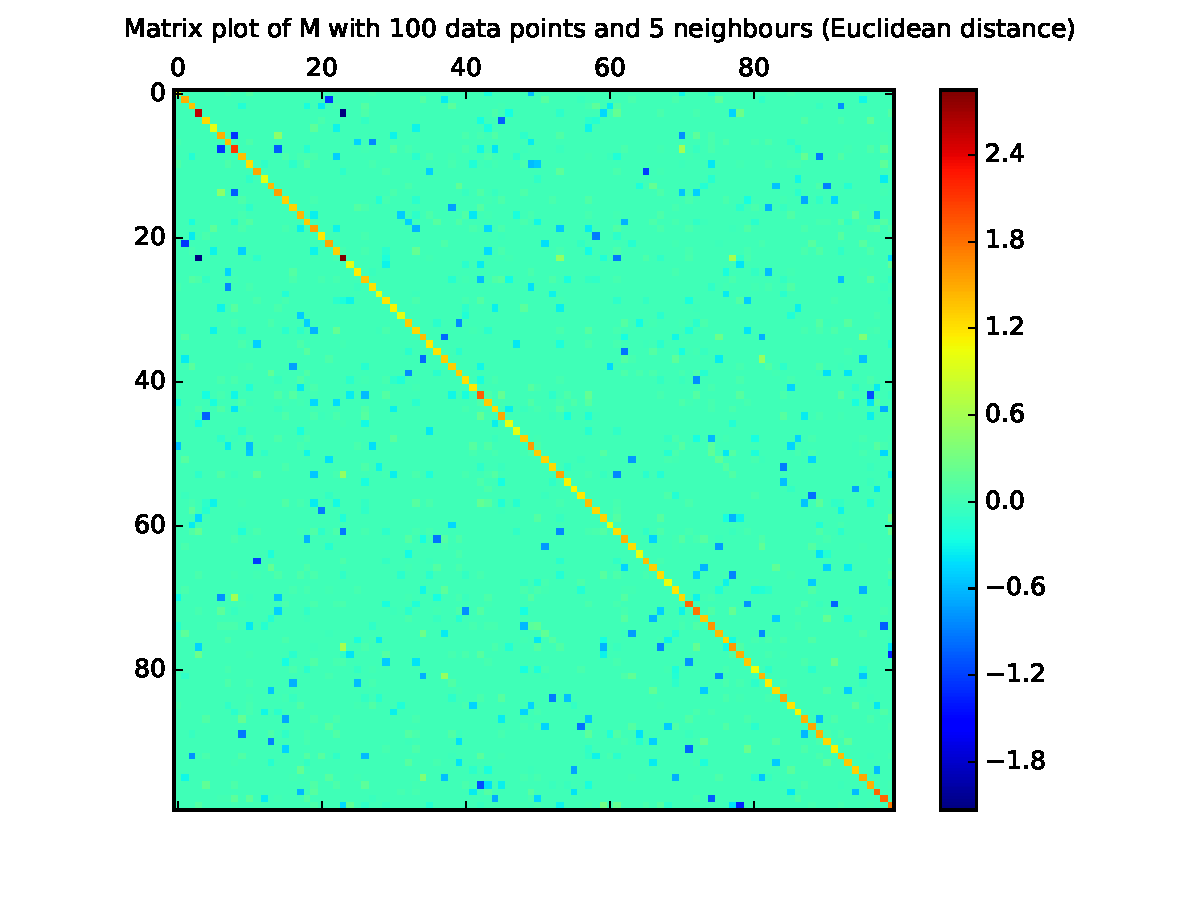
\includegraphics[scale=0.6]{1_figures/matrix_plot}
	\caption{Structure of matrix \textit{M}}
	\label{fig:mat_plot}
\end{figure}
\begin{figure}
	\centering
	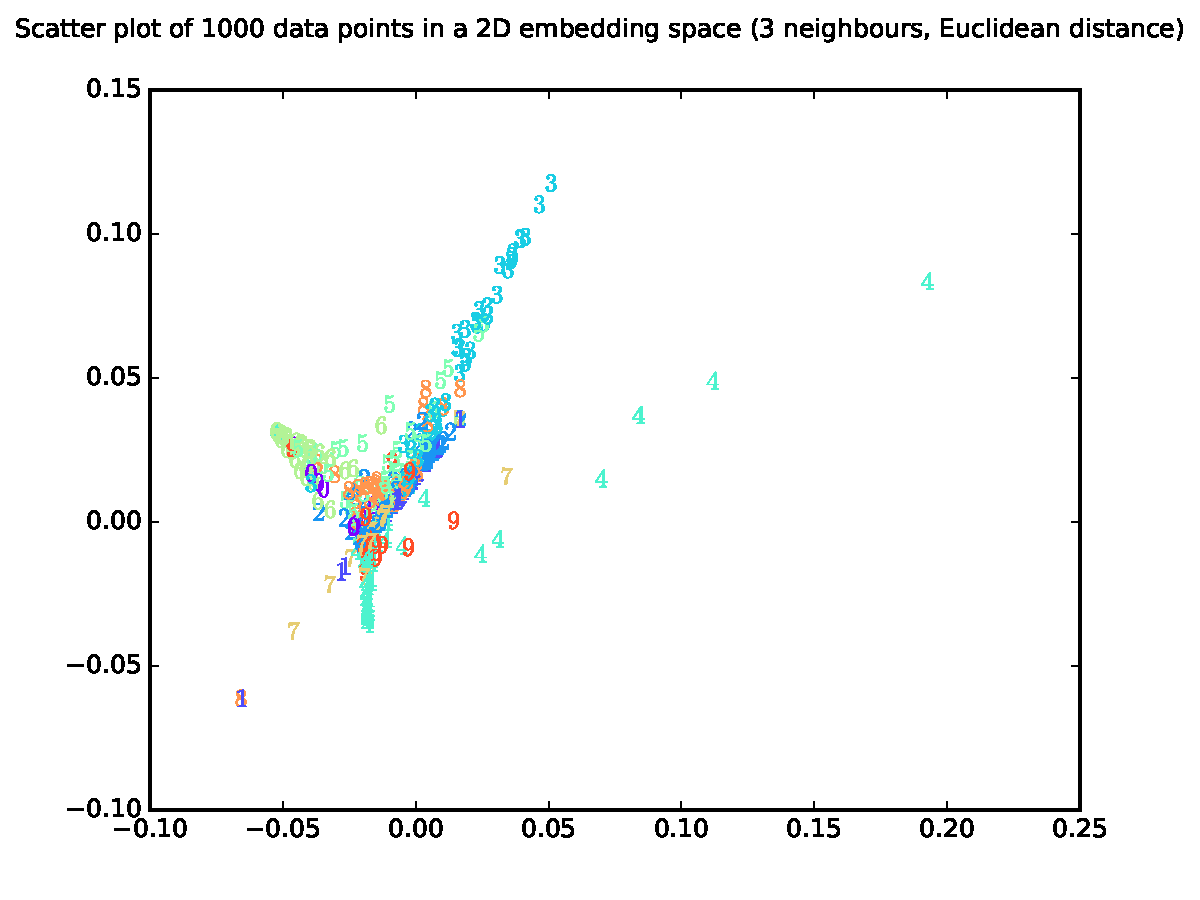
\includegraphics[scale=0.6]{1_figures/2Dembed_3neigh_Euclidean}
	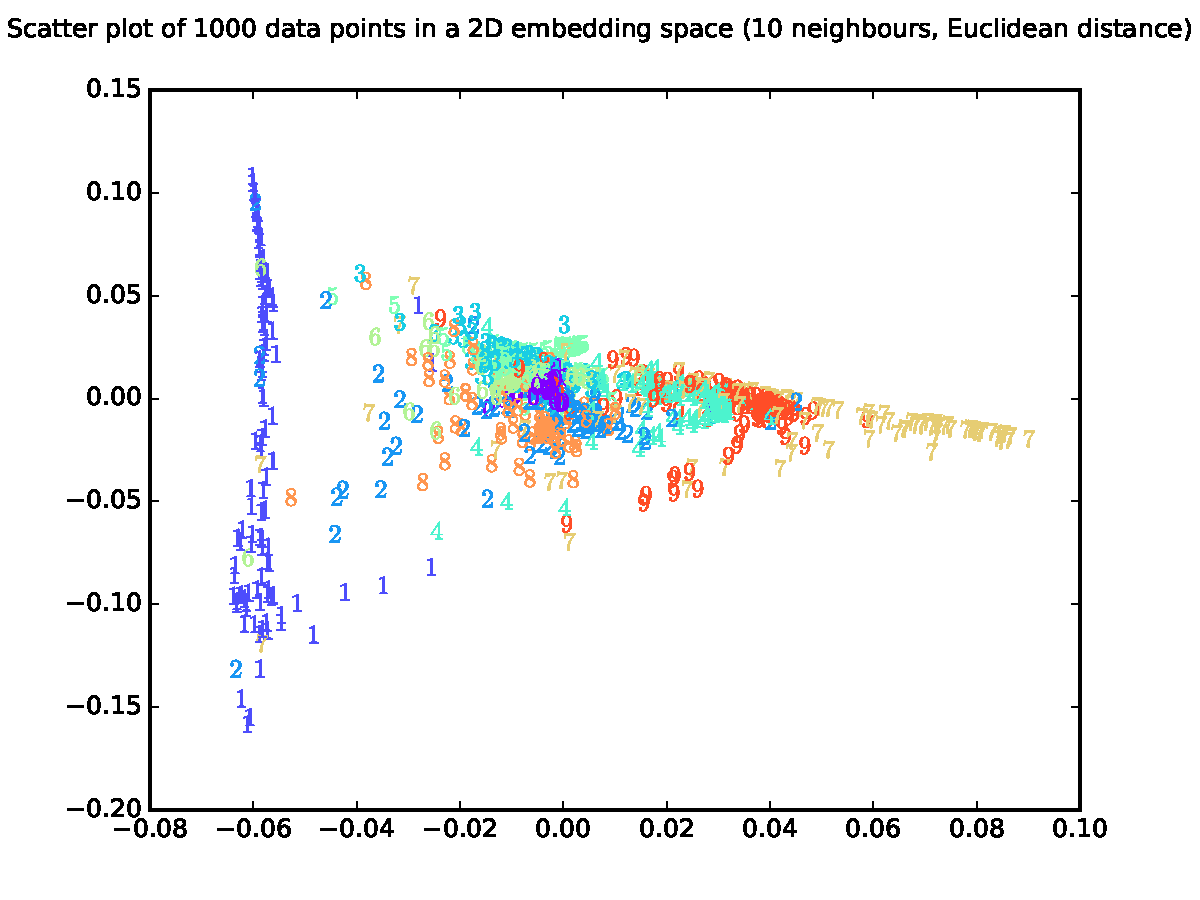
\includegraphics[scale=0.6]{1_figures/2Dembed_10neigh_Euclidean}
	\caption{2D embedding space for different number of neighbours}
	\label{fig:dif_neigh}
\end{figure}
\begin{figure}
	\centering
	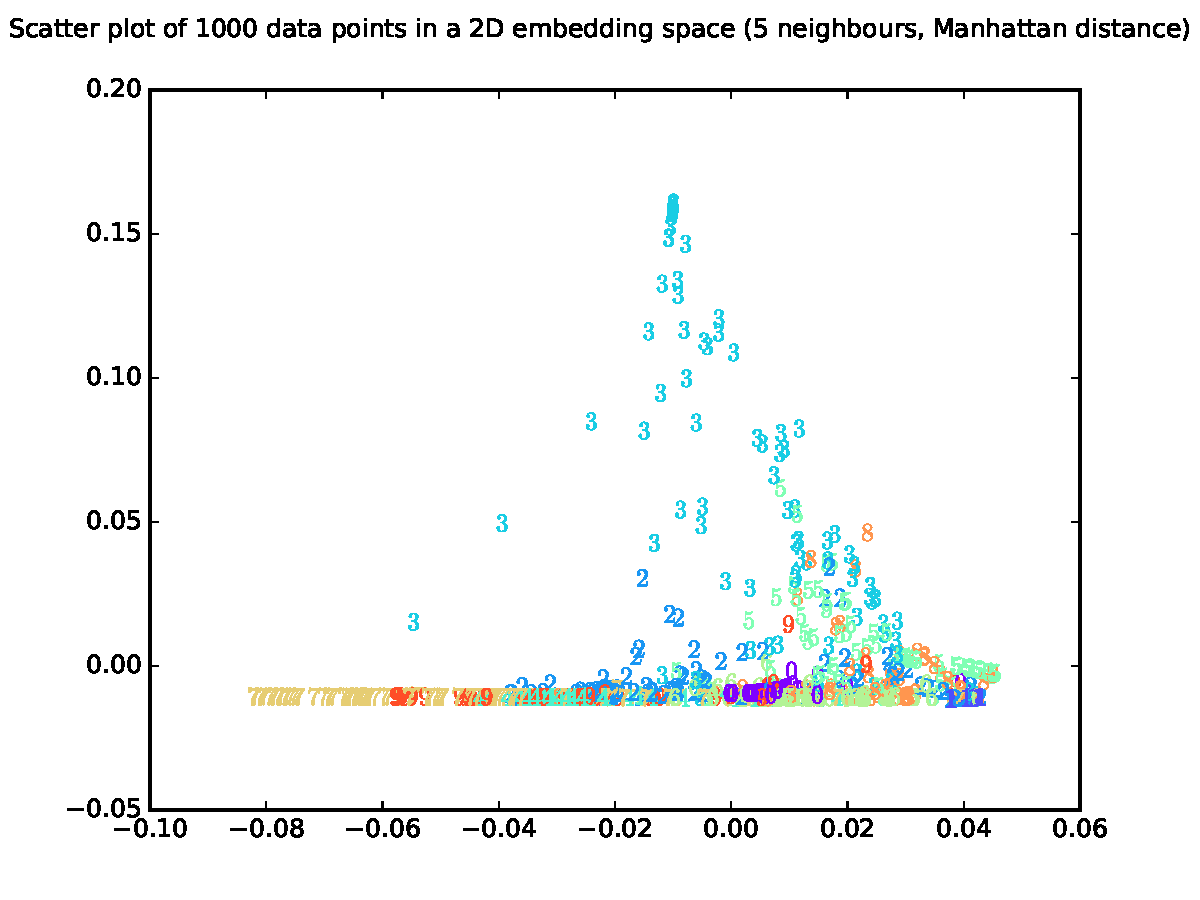
\includegraphics[scale=0.6]{1_figures/2Dembed_5neigh_Manhattan}
	\caption{2D embedding space for Manhattan distance}
	\label{fig:manhattan}
\end{figure}
\begin{figure}
	\centering
	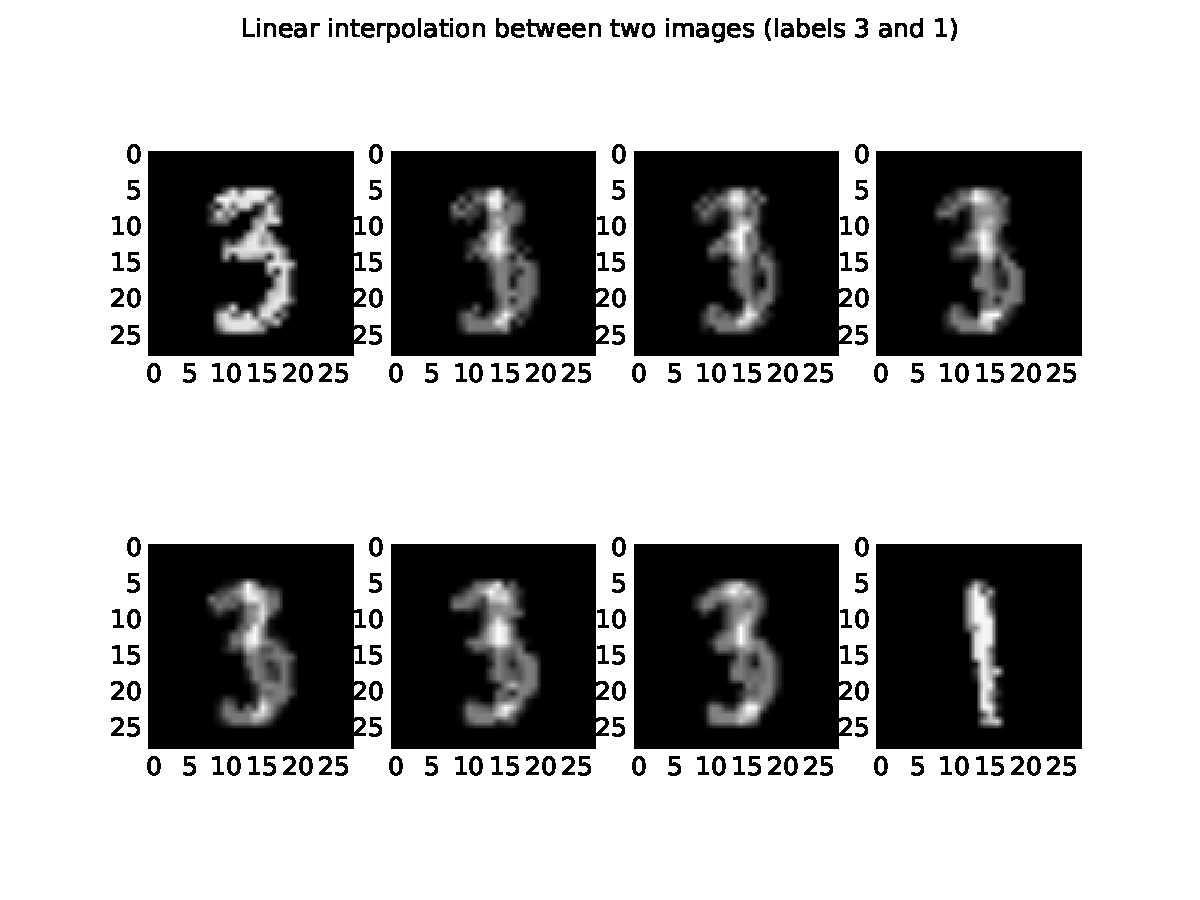
\includegraphics[scale=0.6]{1_figures/linear_int}
	\caption{Linear interpolation in original data space}
	\label{fig:interpolation}
\end{figure}
\end{homeworkProblem}
\clearpage

\end{document}

